\chapter{Experimentos e Resultados}\label{cap:resultados}
Esta seção apresenta os resultados das cinco arquiteturas analisadas. 
Em seguida, a arquitetura com melhor desempenho é analisada mais detalhadamente em diferentes aspectos.
Todos a pesquisa foi realizada em uma máquina com placa gráfica NVIDIA GeForce RTX 3060 Ti, processador Intel Core i7-11700K de 3,60GHz e 16GB de memória RAM.
% ----------------------------------------------------------
\section{Resultados dos Modelos}\label{sec:modelsresults}
%A Tabela \ref{tab:metrics} exibe a acurácia, precisão e revocação das arquiteturas escolhidas. 
%O \acrshort{vit} apresenta o melhor desempenho em termos de acurácia e precisão no conjunto de dados, enquanto sua revocação foi ligeiramente inferior ao do $DenseNet$ e $InceptionV3$, que empataram na melhor revocação. 
%O $MobileNetV3$ obteve a pior revocação e a menor acurácia entr os demais.

% \begin{table}[tb]
% \caption{\label{tab:metrics} Métricas dos diversos modelos}
% \begin{center}
% \begin{tabular}{rrrrr}
% \toprule
%  Modelo & Acurácia &  Precisão & Revocação \\
% \midrule
%      \acrshort{vit} & \textbf{0,83} & \textbf{0,87} & 0,76 \\
%      VGG19 & 0,76 & 0,75 & 0,77 \\
%      DenseNet & 0,79 & 0,79 & \textbf{0,79} \\
%      InceptionV3 & 0,81 & 0,83 & \textbf{0,79} \\
%      MobilenetV3 & 0,75 & 0,80 & 0,67 \\
% \bottomrule
% \end{tabular}
% \end{center}
% \end{table}

A Tabela \ref{tab:metrics} exibe a acurácia de cada modelo com diferentes taxas de aprendizagem usando \acrshort{sgd} como otimizador.
A taxa de aprendizagem de 1x10$^{-5}$ apresentou melhores acurácias no geral, mas não gerou o melhor modelo.
Nenhum modelo obteve boa acurácia com taxa de aprendizagem de 1x10$^{-5}$, indicando que uma taxa muito baixa limitou a capacidade dos modelos de convergir a uma boa resposta.

O \textit{MobileNetV2} obteve os piores resultados com as outras duas taxas de aprendizagem.
Já o \acrshort{vit} apresentou o melhor desempenho, sua acurácia tanto com taxa de aprendizagem de 1x10$^{-3}$ quanto de 1x10$^{-4}$ foram as melhores.

\begin{table}[tb]
\caption{\label{tab:metrics} Acurácia dos cinco modelos com diferentes taxas de aprendizagem.}
%\resizebox{\columnwidth}{!}{%
\begin{center}
\begin{tabular}{c|ccc}
\toprule
\multirow{2}{*}{Modelos} & \multicolumn{3}{c}{Taxa de aprendizagem}   \\
                         & 1x10-03     & 1x10-04     & 1x10-05     \\
\midrule
VGG19                    & 0,808 & 0,732 & 0,524 \\
\midrule
InceptionV3              & 0,795     & 0,731     & 0,529        \\
\midrule
DenseNet                 & 0,802     & 0,658     & 0,592     \\
\midrule
MobileNetV2              & 0,781  & 0,608 & 0,534 \\
\midrule
ViT                      & 0,816     & \textbf{0,826}     & 0,511     \\
\bottomrule
\end{tabular}
\end{center}
%
%}
\end{table}

O desempenho do \textit{MobileNetV2} pode ser explicado por sua arquitetura, projetada para uso em dispositivos com menor poder computacional \cite{mobilenetv2}, possuindo, portanto, um número significativamente menor de parâmetros treináveis em comparação com as outras arquiteturas.

Um comportamento que todos os modelos tiveram, exceto o \acrshort{vit}, foi de ter menor acurácia de acordo com a diminuição da taxa de aprendizagem. 
Isso pode significar que taxa mais baixas não são adequadas para ajustar a grande quantidade da parâmetros em redes profundas.

Apesar de tanto o \acrshort{vgg} quanto o \textit{DenseNet} chegarem a acurácias de 80\%, o \acrshort{vit} mostrou resultados ligeiramente melhores. 
Outro ponto a ser considerado é que enquanto o \textit{InceptionV3} levou 47 minutos para completar seu treinamento, o \acrshort{vit} levou apenas 22 minutos no mesmo conjunto de dados. 
Portanto, o \acrshort{vit} foi escolhido como o modelo a ser utilizado na continuidade deste trabalho.
% ----------------------------------------------------------
\section{Avaliação do melhor modelo}\label{sec:bestmodel}

Após a escolha da arquitetura de melhor depesempenho, outras análises devem ser feitas para saber se é possível melhorar seus resultados e o quão adequado foi seu treinamento.

\subsection{Diminuição da intensidade luminosa}
Após a escolha da arquitetura de melhor desempenho, diferentes valores para nesta dissertação denomidado de fator de brilho (\textit{FB}), conforme mencionado em \ref{subsec:datapreprocessing}, foram avaliados usando o \acrshort{vit}, a fim de analisar se o modelo poderia ser aprimorado, levando em consideração o brilho excessivo em algumas imagens.

A Tabela \ref{tab:brightnessfactor} mostra o desempenho do \acrshort{vit} com quatro valores diferentes para \textit{FB}, onde o valor 1 para \textit{FB} significa que a intensidade luminosa da imagem não foi alterada, ou seja a quantidade de regiões com pixeis na cor branca permanece a original. 
Reduzir o \textit{FB} melhorou gradualmente o desempenho do modelo, porém um \textit{FB} muito baixo impactou negativamente o modelo, como mostram os resultados com \textit{FB} igual a 0,25. Reduzir o \textit{FB} para 0,75 melhorou os resultados marginalmente, no entanto, a escolha inicial de 0,5 mostrou-se a melhor entre os valores testados.

\begin{table}[tb]
\caption{\label{tab:brightnessfactor} Redução de áreas de brancos e desempenho do \acrshort{vit}}
\begin{center}
\begin{tabular}{c|ccc}
\toprule
 Fatores de brilho & Acurácia &  Precisão  & Revocação \\
\midrule
     0,25 & 0,703 & 0,758 & 0,604 \\
     0,5 & \textbf{0,826} & \textbf{0,863} & \textbf{0,778} \\
     0,75 & 0,769 & 0,802 & 0,738 \\
     1 & 0,756 & 0,782 & 0,708 \\
\bottomrule
\end{tabular}
\end{center}
\end{table}

\subsection{Curvas de acurácia e perda do melhor modelo}
A Fig. \ref{fig:acc} e a Fig. \ref{fig:loss} mostram o \acrshort{vit} atuando em seu treinamento (linha azul) e validação (linha vermelha).

No treinamento, a acurácia (Fig. \ref{fig:acc}) converge para 0,87, enquanto na validação permanece em aproximadamente 0,83. No entanto, ao analisar apenas a acurácia no conjunto de validação, podemos observar que ela começou com valores relativamente altos antes de convergir. A pequena discrepância entre a acurácia de treinamento e validação indica que não houve $overfitting$ dos dados, e o modelo conseguiu criar uma boa generalização.

Analisando a perda (loss) (Fig. \ref{fig:loss}) durante o treinamento, podemos ver que, apesar da alta acurácia no conjunto de treino, a perda ainda era relativamente alta antes de se estabilizar em torno de 0,37 (linha vermelha), enquanto o conjunto de validação se estabilizou em 0,43 (linha azul).

\begin{figure}[tb]
\centerline{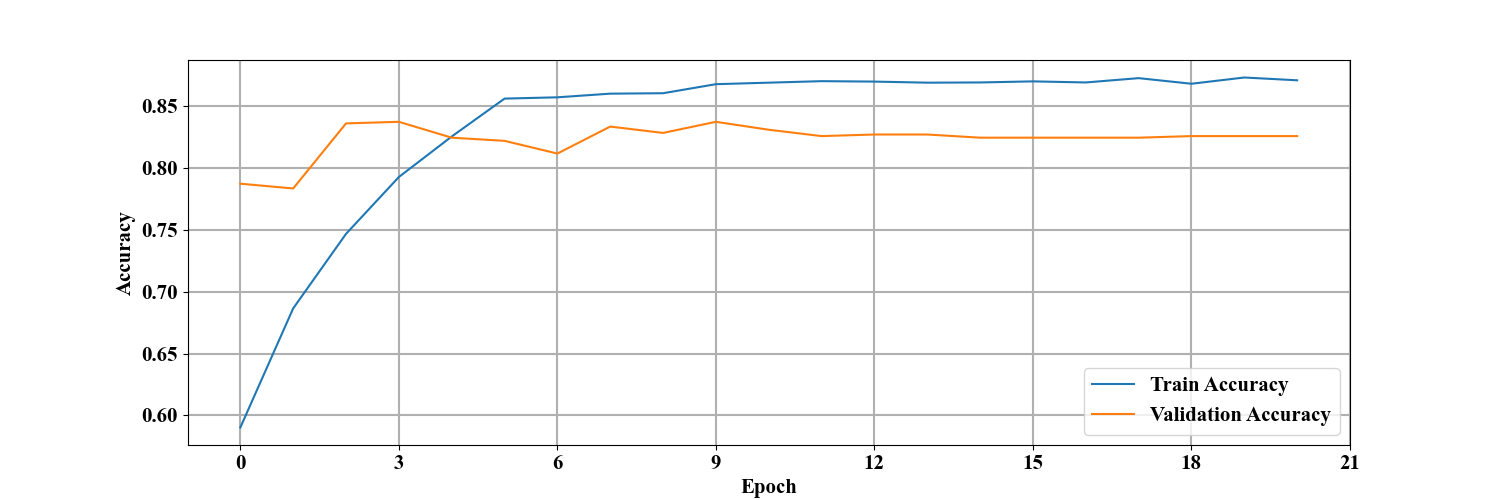
\includegraphics[width=1\linewidth]{images/resultados/sgd_accuracy.png}}
\caption{Acurácia do \acrshort{vit} durante treino e validação.}
\label{fig:acc}
\end{figure}

\begin{figure}[tb]
\centerline{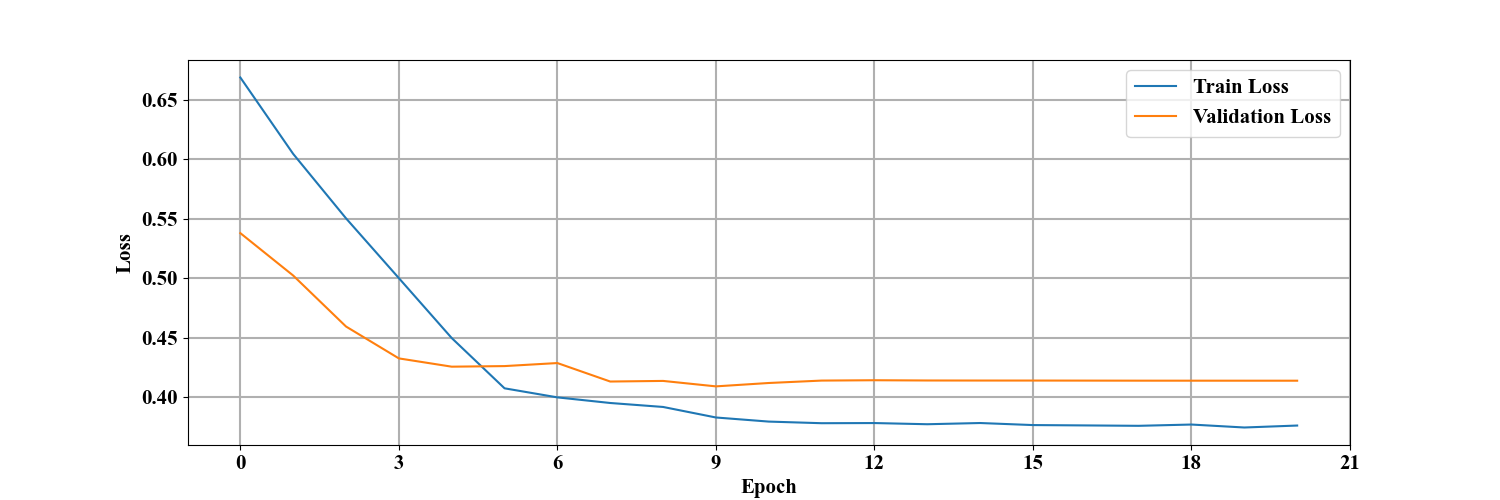
\includegraphics[width=1\linewidth]{images/resultados/sgd_loss.png}}
\caption{Perda do \acrshort{vit} durante treino e validação.}
\label{fig:loss}
\end{figure}

A pequena diferença na acurácia entre os conjuntos de treinamento e validação (Fig. \ref{fig:acc}) pode ser justificada pela introdução de 
características no conjunto de validação que não estão presentes no conjunto de treinamento. 
%Devido ao considerável número de imagens capturadas durante a chuva, uma quantidade não negligenciável de imagens apresenta problemas de nitidez. 
%seja devido à lente da câmera estar molhada ou devido à alta reflexão de luz em poças de água na rua.
% ----------------------------------------------------------
\subsection{Melhor modelo com diferentes quantidades de câmeras}\label{sec:cameraquantity}

Com o objetivo de verificar se aumentar a quantidades de câmeras no conjunto de treino levaria a melhorias significativas de sua performance, 
a arquitetura \acrshort{vit} foi treinada com conjuntos de treinos menores. 
Esses conjuntos de treino possuem menores quantidades de câmeras, mas mantêm a quantidade de imagens por classe para cada câmera.
Para montar estes conjuntos a serem comparados ao utilizado, entre as 60 câmeras que compõem o original foram escolhidas aletoriamente 30 câmeras para montar o segundo conjunto.
Dessas 30 câmeras foram selecionadas aleatoriamente 15 câmeras para formar o terceiro conjunto.
Dessa forma, todos os três conjuntos de treinos possuem as mesmas 15 câmeras, e o efeito de adicionar novas câmeras ao conjunto pode ser mais facilmente compreendido.
A Tabela \ref{tab:trainingimages} mostra a relação entre o tamanho do conjunto de treino, sua acurácia e tempo de treino. 
O modelo foi testado no mesmo conjunto de teste que faz parte do conjunto de dados original.

\begin{table}[!ht]
\begin{center}
\caption{Acurácia $\times$ tempo de treino $\times$ número de imagens usadas}
\label{tab:trainingimages}
\begin{tabular}{c|cc}
%\hline
\toprule
\textbf{\textbf{Nº de Câmeras}} & \textbf{Acurácia} & \textbf{Tempo (minutos)}\\
%\hline\hline
\midrule
15 &  0,728 & 17\\
30 & 0,804 & 18 \\
60 & 0,826 & 21 \\
%\hline
\bottomrule
\end{tabular}
\end{center}
\end{table}

Como esperado, aumentar a diversidade de câmeras no conjunto de treino e, consequentemente, aumentar a quantidade de imagens de treino aumentou a acurácia do modelo. 
Entretanto, o número utilizado está completamente adequado pois adicionar mais câmeras não traria melhorias significativas na performance, 
visto que dobrando a quantidade de imagens de 1800 para 3600, ou seja, dobrando de 30 câmeras para 60 câmeras no conjunto de treino, somente representou uma melhoria de 0,022 na acurácia.

% ----------------------------------------------------------
\section{Comparação entre diferentes otimizadores}\label{sec:optimizer}
Apesar de inicialmente todos os modelos serem treinados utilizando \acrshort{sgd} como otimizador, 
a escolha de diferentes otimizadores com diferentes taxas de aprendizado podem afetar a performance da \acrshort{cnn}. 

Baseado nos resultados de Dogo \textit{et al.} \cite{Dogo2022optimizers}, onde diferentes otimizadores foram comparados com redes neurais e conjuntos de dados de diferentes tamanhos e complexidades, 
essa dissertação comparou os resultados no \acrshort{vit} com \acrshort{sgd}, \acrlong{adam}\cite{adam} e o \acrlong{nadam}\cite{nadam}. 
Todos os otimizadores utilizaram as mesmas configurações descritas na seção \ref{sec:methodology_models}, com diferentes taxa de aprendizado iniciais.

\begin{table}[tb]
%\resizebox{\columnwidth}{!}{%
\caption{\label{tab:optimizer_acc} Acurácia do \acrshort{vit} com diferentes otimizadores.}
\begin{center}
\begin{tabular}{c| c c c }
\toprule
\multirow{2}{*}{\begin{tabular}[c]{@{}c@{}}Taxa de \\ Aprendizado\end{tabular}} & \multicolumn{3}{c}{Acurácia}   \\
                                                                                & SGD      & Adam     & NAdam    \\
\midrule
1x10-06                                                                           & 0,504   & 0,833 & 0,819 \\
1x10-05                                                                           & 0,512 & 0,841 & \textbf{0,862} \\
1x10-04                                                                           & 0,826 & 0,636 & 0,650    \\
\bottomrule
\end{tabular}
\end{center}%
%}
\end{table}

\begin{figure}[tb]
\centerline{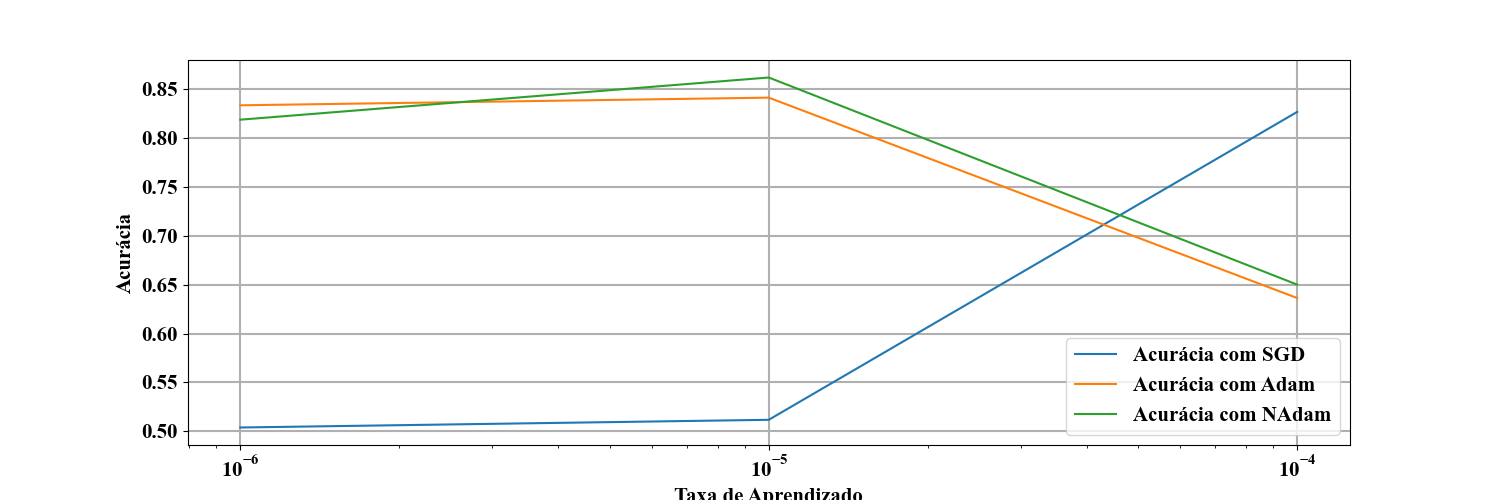
\includegraphics[width=1\linewidth]{images/resultados/optimizer_acc.png}}
\caption{Acurácia do \acrshort{vit} com diferentes otimizadores.}
\label{fig:optmizer_acc}
\end{figure}

Os resultados mostram que ambos \acrshort{adam} e \acrshort{nadam} possuíram acurácias melhores que o \acrshort{sgd}. 
O \acrshort{nadam} obteve a melhor acurácia: 0,86 com taxa de aprendizado de 1x10$^{-5}$.
Avaliando o \acrshort{sgd}, taxas de aprendizado menores obtiveram piores resultados, provavelmente indicando que o passo foi muito pequeno para sair de mínimos locais, especialmente em uma arquitetura mais complexa como o \acrshort{vit}. 

Nenhum dos otimizadores conseguiu boa performance com a taxa de aprendizado mais baixa, 
que pode ser explicado pelo modelo não ter feito atualizações significativas em seus pesos durante o treino.
As duas versões do \acrshort{adam} obtiveram melhor performance com uma taxa de aprendizado mais moderada, com o \acrshort{nadam} se sobressaindo. 
A utilização da aceleração de Nesterov para atualizações mais rápidas pelo \acrshort{nadam} pode ser o responsável pelo melhor desempenho.

As Figuras \ref{fig:nadam_acc} e \ref{fig:nadam_loss} mostram a acurácia e perda do \acrshort{vit} durante treino 
usando o \acrshort{nadam} com taxa de aprendizagem de 1x10$^{-5}$, onde a maior acurácia de validação foi obtida.
Levando em consideração que o modelo estabilizou sua acurácia de treino em 100\% enquanto a acurácia de validação ficou em volta de 86\%,
indica que o modelo não conseguiu generalizar bem os dados, indicando \textit{overfitting}.
Isso é corroborado pela curva de perda, onde a perda na validação aumentou, em contraste com a diminuição para quase zero da perda de treino.

\begin{figure}[tb]
\centerline{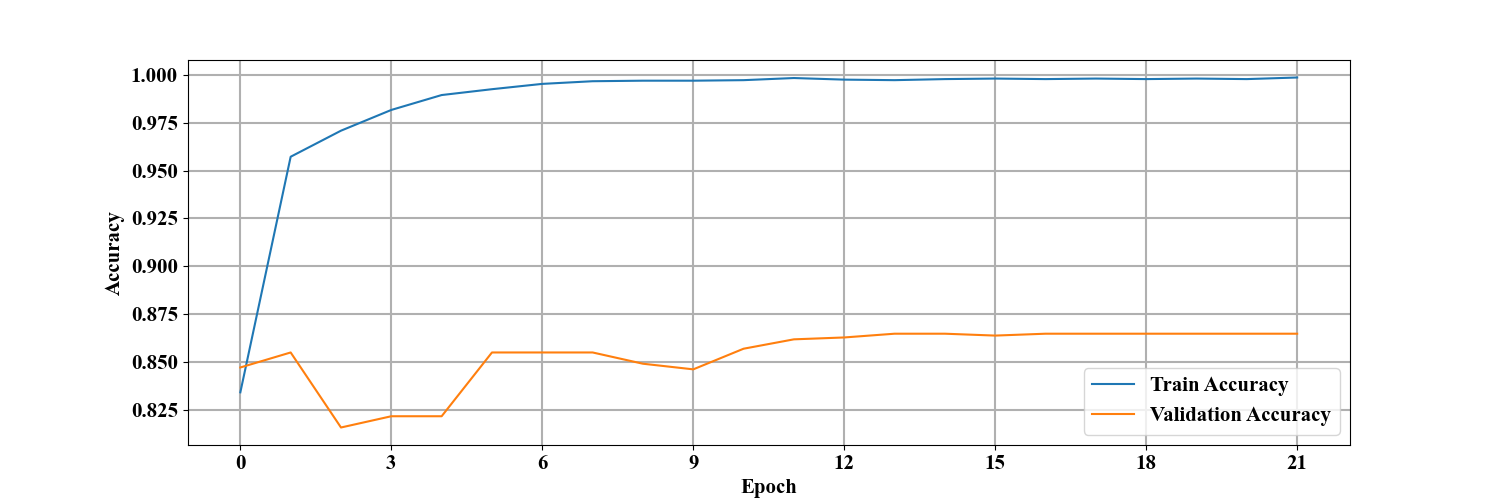
\includegraphics[width=1\linewidth]{images/resultados/nadam_accuracy.png}}
\caption{Acurácia do \acrshort{vit} com NAdam.}
\label{fig:nadam_acc}
\end{figure}

\begin{figure}[tb]
\centerline{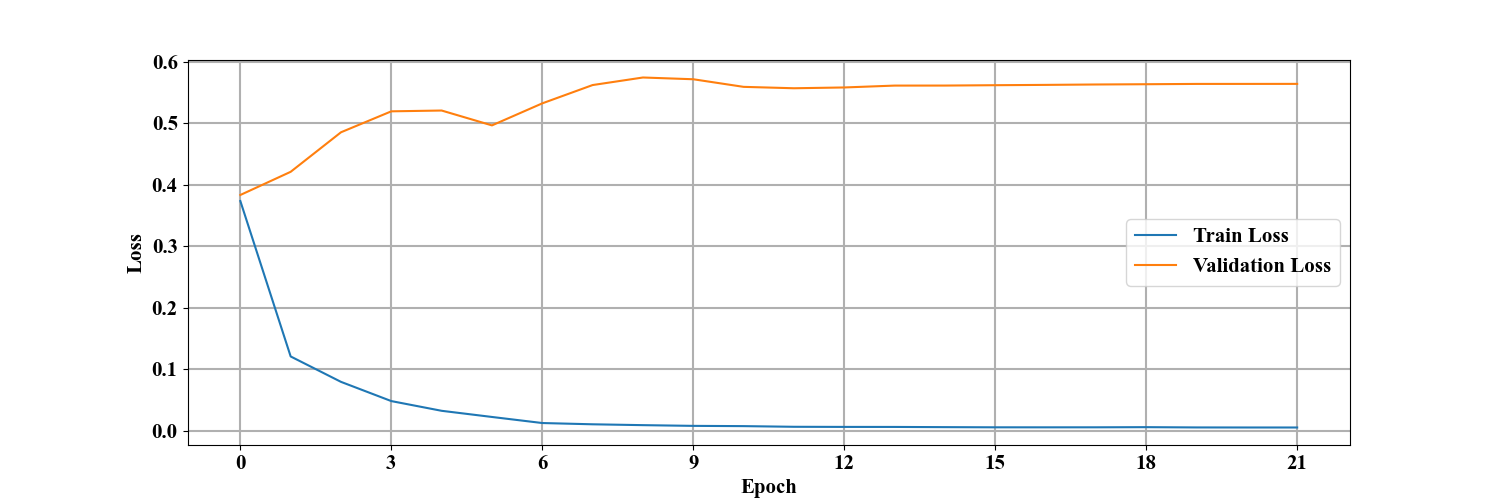
\includegraphics[width=1\linewidth]{images/resultados/nadam_loss.png}}
\caption{Perda do \acrshort{vit} com NAdam.}
\label{fig:nadam_loss}
\end{figure}

Fazendo a mesma análise para a taxa de aprendizagem de 1x10$^{-6}$, onde a acurácia de validação foi um pouco menor, pode-se notar algumas semelhanças e diferenças.
Ainda houve uma diferença significativa entre as acurácias de treino e validação, onde a acurácia de treino estabilizou por volta de 98\%, enquanto a acurácia de validação ficou em 82\%.

Entretanto, a curva de perda mostrou melhorias. 
Tanto a curva de treino quanto a curva de validação tenderam a diminuir, apesar de que a diminuição da perda na validação não ser tão significativa.
Este modelo não mostrou sinais claros de \textit{overfitting} como o modelo com maior taxa de aprendizagem, mas ainda demonstra sinais de melhorias.

\begin{figure}[tb]
     \centerline{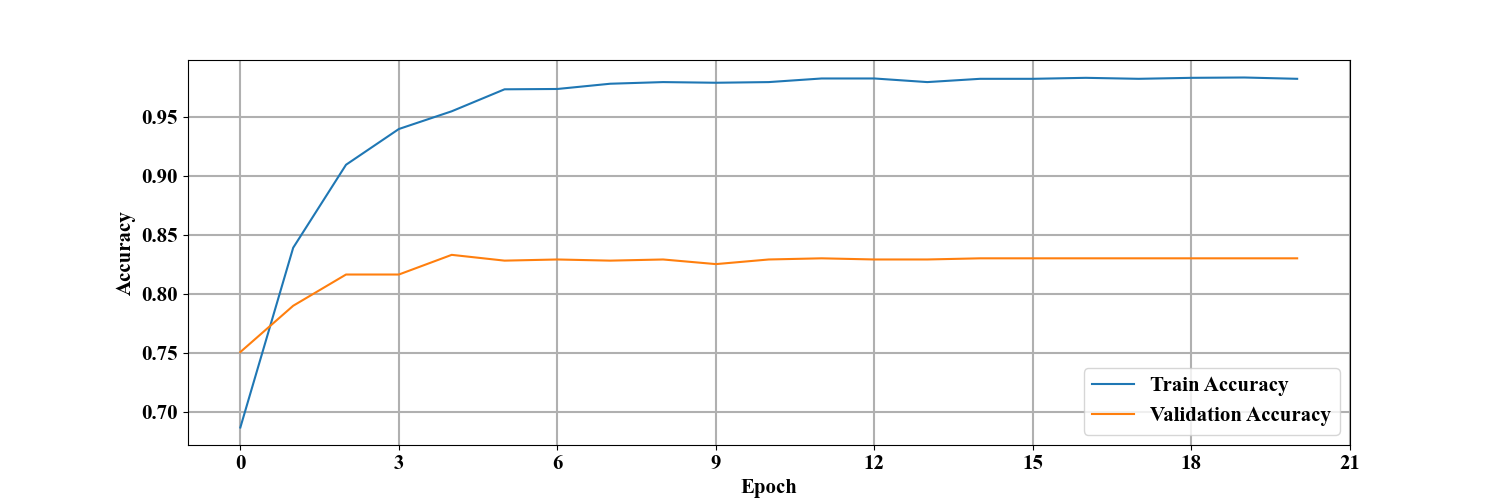
\includegraphics[width=1\linewidth]{images/resultados/nadam_accuracy_1e06.png}}
     \caption{Acurácia do \acrshort{vit} com NAdam e menor taxa de aprendizagem.}
     \label{fig:nadam_acc_1x1006}
\end{figure}
     
\begin{figure}[tb]
     \centerline{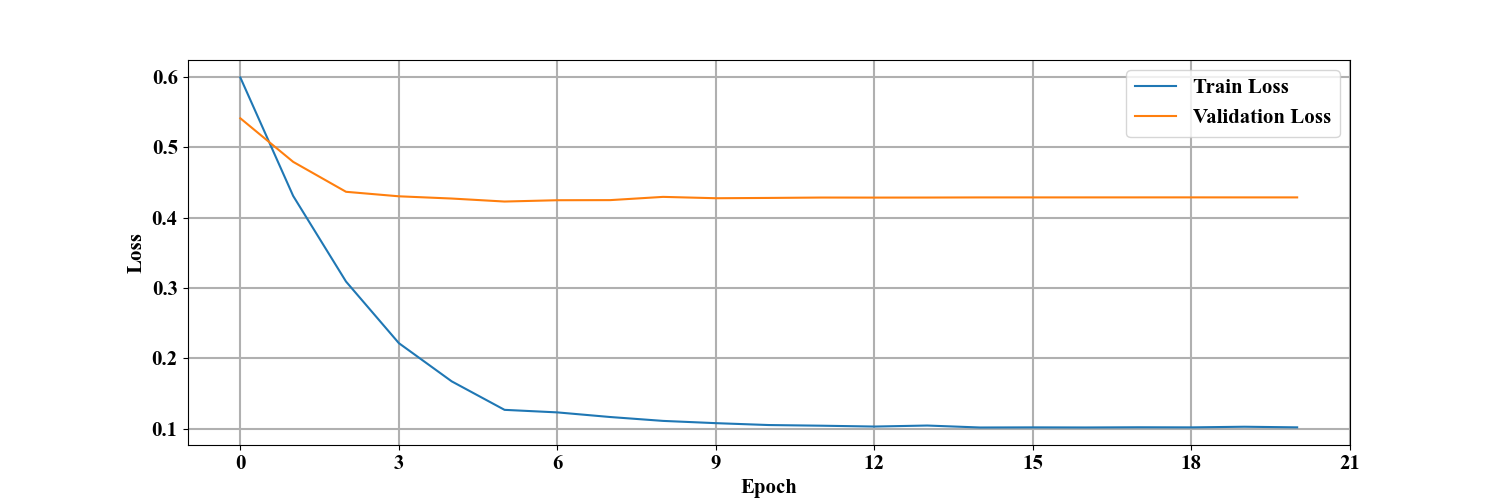
\includegraphics[width=1\linewidth]{images/resultados/nadam_loss_1e06.png}}
     \caption{Perda do \acrshort{vit} com NAdam e menor taxa de aprendizagem.}
     \label{fig:nadam_loss_1x1006}
\end{figure}

Visto que o modelo \acrshort{vit} usando \acrshort{nadam} e taxa de aprendizagem de 1x10$^{-6}$ obteve acurácia de validação semelhante a do modelo com o \acrshort{sgd} de taxa de aprendizagem de 1x10$^{-4}$,
entretanto, teve maior diferença entre as acurácias de treino e validação, assim como redução na função de perda, o modelo com \acrshort{sgd} vai continuar a ser analisado como o melhor modelo, por possuir maior estabilidade.
% As Figuras \ref{fig:adam_acc} e \ref{fig:adam_loss} mostram a acurácia e perda do \acrshort{vit} durante treino usando o \acrshort{adam}.

% \begin{figure}[tb]
% \centerline{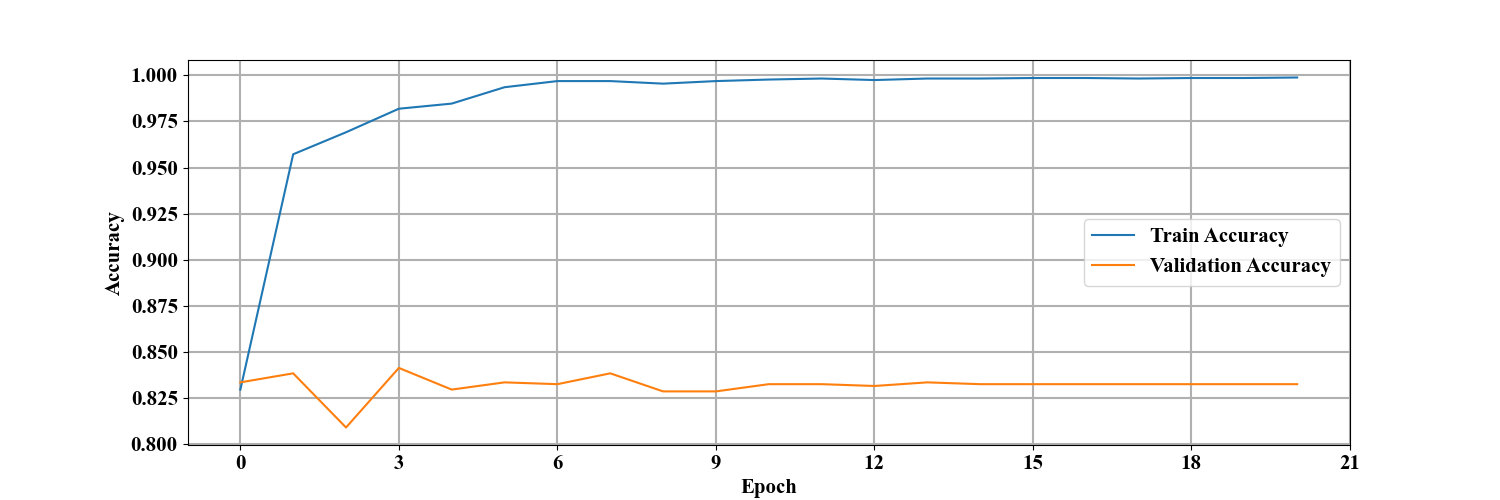
\includegraphics[width=1\linewidth]{images/resultados/adam_accuracy.png}}
% \caption{Acurácia do \acrshort{vit} durante treino e validação com Adam.}
% \label{fig:adam_acc}
% \end{figure}

% \begin{figure}[tb]
% \centerline{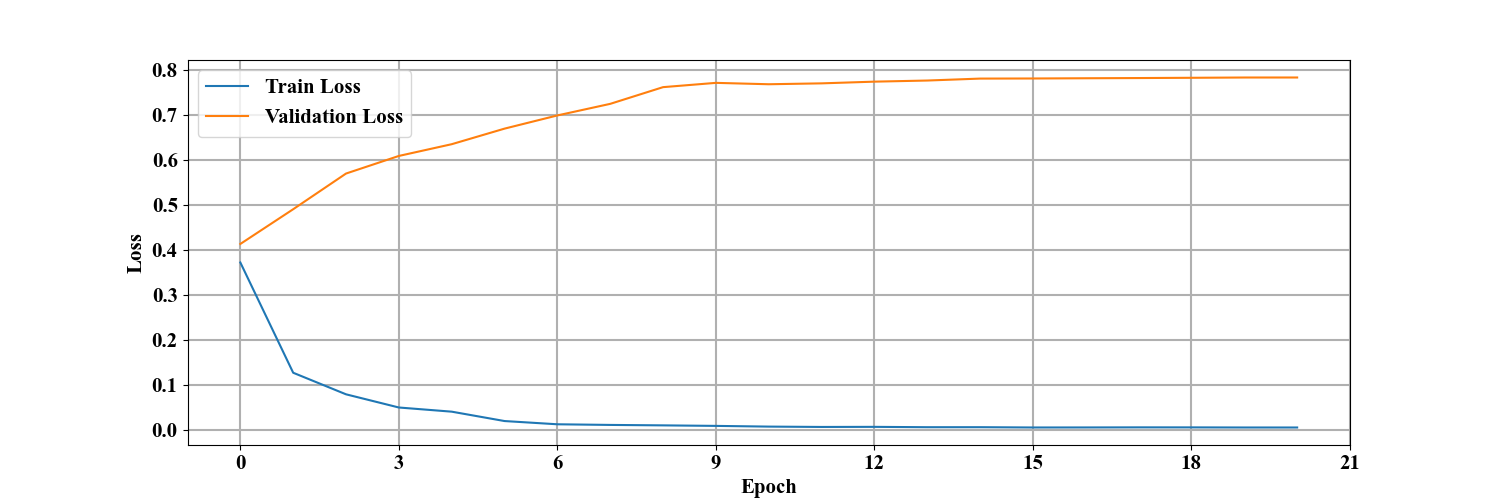
\includegraphics[width=1\linewidth]{images/resultados/adam_loss.png}}
% \caption{Perda do \acrshort{vit} durante treino e validação com Adam.}
% \label{fig:adam_loss}
% \end{figure}
% ----------------------------------------------------------
\section{Comparações entre cena diurna e noturna}

Para melhor entender a iluminação da cena nos resultados da classificação do modelo \cite{piedad2022}, 
o melhor resultado do \acrshort{vit} com o \acrshort{sgd} descrito na seção \ref{sec:optimizer} foi avaliado em relação a suas métricas com a luz do dia e com luzes noturnas no local, 
com os resultados mostrados na tabela \ref{tab:daynight_acc}.

\begin{table}[tb]
%\resizebox{\columnwidth}{!}
\end{center}
\end{table}

% \begin{table}[tb]
% %\resizebox{\columnwidth}{!}{%
% \caption{\label{tab:daynight_acc} Métricas do \acrshort{vit} ao longo do dia.}
% \begin{tabular}{c|cccccc}
% \toprule
% \multirow{2}{*}{Otimizador} & \multicolumn{3}{c}{Diurna}         & \multicolumn{3}{c}{Noturna}       \\
%                             & Acurácia & Precisão & Revocação & Acurácia & Precisão & Revocação \\
% \midrule
% SGD                         & 0,802 & 0,702 & 0,694  & 0,758 & 0,800 & 0,758  \\
% \midrule
% NAdam                       & 0,839 & 0,820 & 0,656  & 0,850 & 0,916 & 0,807  \\
% \bottomrule
% \end{tabular}%
% %}
% \end{table}

Em contraste com os resultados apresentados e descritos no capítulo \ref{cap:trabalhos}, 
onde o modelo apresentou resultados substancialmente melhores em imagens diurnas em comparação com imagens noturnas \cite{piedad2022},
o modelo treinado no conjunto de dados do \acrshort{cor} obteve menores diferenças na acurácia entre imagens diurnas e noturnas.
Essa maior estabilidade da acurácia pode ser explicada pela redução do brilho da imagem através do pré-processamento realizado.
%, onde as imagens diurnas com céu mais claro foram escurecidas, semelhando-se a imagens noturnas.
% ----------------------------------------------------------
\section{Outros conjuntos de dados}\label{sec:resultados_outros}

O modelo \acrshort{vit} treinado no conjunto do COR também foi testado em dois outros conjuntos de dados, 
o \acrfull{efd} \cite{BarzSchroeterMuench2018_1000117723} e o conjunto de dados de Sazara \textit{et al.} \cite{sazara2019}.
O \acrshort{efd} é composto de 327 imagens de normalidade e 252 imagens de alagamento para um total de 579.
O conjunto de dados de Sazara \textit{et al.} possui 491 imagens, onde 238 são de normalidade e 253 são imagens de alagamento.

Podemos ver na Tabela \ref{tab:vitperformance} que o desempenho do modelo diminuiu em diferentes conjuntos de dados. 
Apesar do aumento da precisão, houve uma queda muito grande na acurácia, mostrando que o modelo não conseguiu generalizar tão bem em imagens com diferentes ângulos, qualidade e iluminação.

\begin{table}[tb]
\caption{\label{tab:vitperformance} Performance do \acrshort{vit} em outros conjuntos de dados}
\begin{center}
\begin{tabular}{c|cccc}
\toprule
 Conjunto de Dados & Acurácia & Precisão & Revocação \\
\midrule
     COR & 0,826 & 0,863 & 0,778 \\
     EFD & 0,731 & 0,892 & 0,714 \\
     Sazara & 0,744 & 0,903 & 0,674 \\
\bottomrule
\end{tabular}
\end{center}
\end{table}